% !TEX root = main.tex

%%%%%%%%%%%%%%%%%%%%%%%%%%%%%%%%%%%%%%%%%%%%%%%%%%%%%%%%%%%%%%%%%%%%%%%%%%%%%%%%%%%%%%%%%%%%%%%%
\section{測定}
%%%%%%%%%%%%%%%%%%%%%%%%%%%%%%%%%%%%%%%%%%%%%%%%%%%%%%%%%%%%%%%%%%%%%%%%%%%%%%%%%%%%%%%%%%%%%%%%

\subsection*{測定機器}
コイル,キャパシタ,固定抵抗,ブレッドボード,オシロスコープ,発振器,配線材料,関数電卓,ノートPC

\subsection*{測定手順}
\subsubsection*{理論値計算}
指定された$L,C,R$の値をもとにインピーダンスの理論値を$f = 100$\,[Hz]\sim 100\,[kHz]
の範囲で回路シミュレータを用いて計算し,インピーダンスの大きさ,偏角,電流相対比の
理論曲線をそれぞれ両対数・片対数・通常方眼グラフ用紙にプロットする.
なお,理論値計算では一律にコイルの巻線抵抗を$r_L = 0.6$\,[\Omega]に設定すること.
共振周波数$f_0$\,[Hz],同調度計算のための$f_L,f_H$\,[Hz]は回路シミュレータから
数値的に求めておく.電流相対比のグラフは$f_L,f_H$を含むよう適切に計算帯域を設定せよ.

\subsubsection*{回路}
測定においては,共振回路全体を流れる電流$I$を測定するために測定用の抵抗$R^{\prime}$を直列に
挿入し,図2に示す回路構成をとる.

\begin{figure}[H]
    \begin{center}
        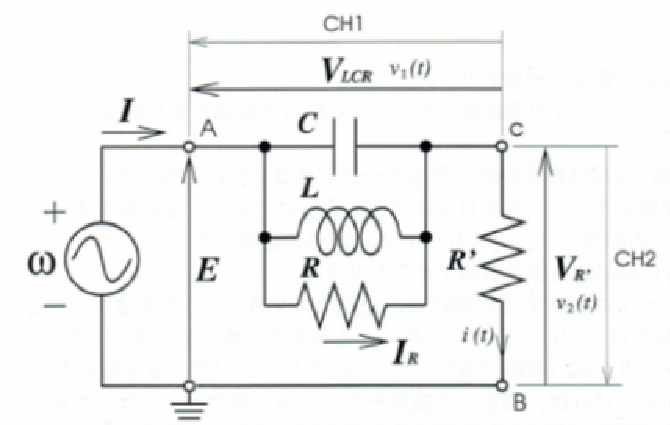
\includegraphics[]{figure2.pdf}
        \caption{LCR並列共振測定回路}
    \end{center}
\end{figure}

\newpage

\subsubsection*{測定1}
発振器から正弦波を発生させ,適当な$R^{\prime}$を用いて図のc点を電圧測定の基準として
$A-c$間$v_1(t)$\,[V]をオシロスコープのCH1,$B-c$間$v_2(t)$\,[V]をCH2で測定する.
回路を流れる瞬間電流値$i(t)$は$i(t)= -v_2 (t)/R^{\prime}$で求まるが,波形が反転している
ことに注意すること.一つの測定周波数$f$\,[Hz]についての測定対象は,
瞬間電圧$v_1(t)$と$v_2(t)$の最大振幅$|V_1|$,$|V_2|\,[\si{\volt}]$,周期$f$\,[Hz],$v_1(t)$と$v_2(t)$の対応する零交差点の
時間幅$ΔT$\,[sec]である.前者二つの振幅値からインピーダンスの大きさを求める.
後者二つの時間幅からインピーダンスの偏角を求める.周波数fはオシロスコープの測定機能を
利用する.測定範囲内で適切に測定し,インピーダンスの周波数特性,電流相対比をそれぞれ
理論値をプロットしたグラフ用紙に記入する.なお,実際の共振周波数$f_0$と$f_L,f_H$を求める
ため,$f_0,f_L,f_H$近傍は詳しく測定すること.

\subsubsection*{実験条件}
使用する素子の条件は$L = 1\,\si{mH},C = 1\,\si{\mu F},R = 22\,\si{k\Omega}$である.

\subsubsection*{使用機器}
\begin{enumerate}
    \item RC発振器(ケンウッド\quad AG-203A)
    \item DSO(Tektronix\quad TBS1022)
    \item ブレッドボード
    \item Qucs\quad 0.0.16
\end{enumerate}

作成した回路を図3に示す.

\begin{figure}[H]
    \begin{center}
        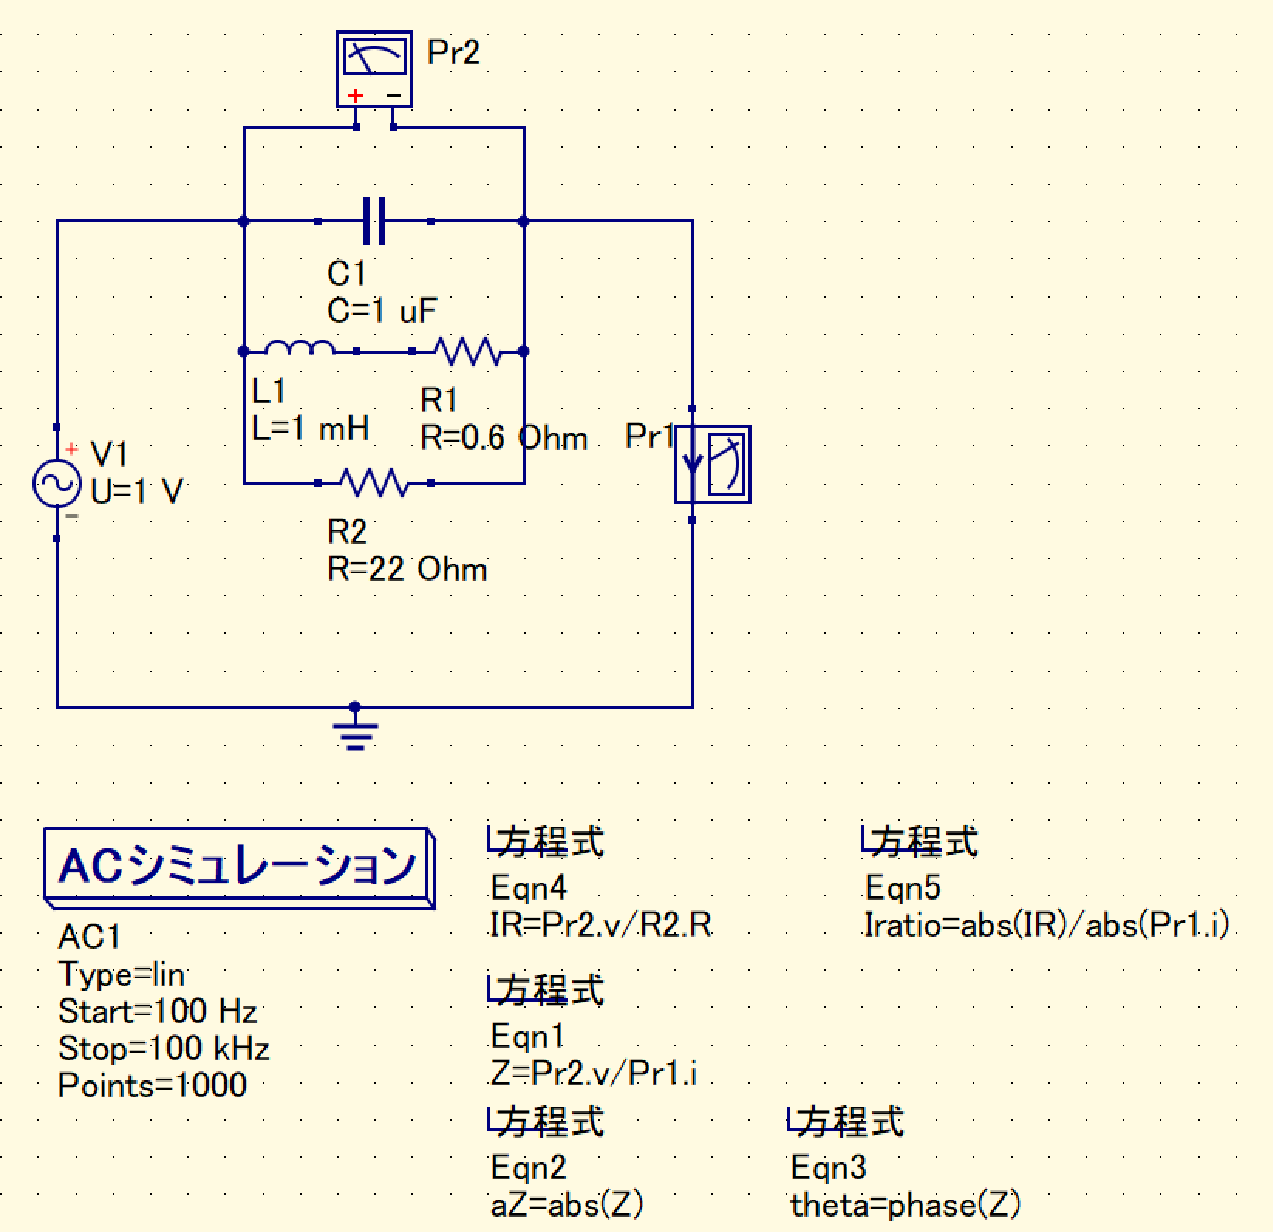
\includegraphics[scale=0.5]{figure3.pdf}
        \caption{作成した回路}
    \end{center}
\end{figure}